\documentclass{standalone}
\usepackage{ tikz }
\usepackage{ xparse }
\usepackage{../../macros}
\usepackage{amssymb}

\usetikzlibrary{shapes.gates.logic.US}

\begin{document}
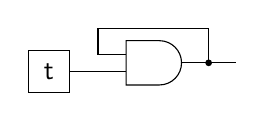
\begin{tikzpicture}[yscale=-1,x=1em,y=1.25em]
        

    \node [draw, minimum width=1.5em, minimum height=1.5em, anchor=east] at (-1,0.75) {$\mathsf{t}$};
    \draw (-1,0.75) -- (1,0.75);
    \node [draw, and gate US, minimum width=2em, minimum height=1.5em, anchor=west] at (1,0.5) {};
    \draw (3,0.5) -- (5,0.5);
    \filldraw (4,0.5) circle (1pt);
    \draw (4,0.5) -- (4,-0.5) -- (0,-0.5) -- (0,0.25) -- (1,0.25);

\end{tikzpicture}
\end{document}